\documentclass[11pt,a4paper]{article}
\usepackage[margin=25mm]{geometry}
\usepackage[T1]{fontenc}
\usepackage[utf8]{inputenc}
% lmodern not available: Computer Modern via T1 (cm-super) or fallback
\usepackage{microtype}
\microtypesetup{expansion=false}
\usepackage{amsmath,amssymb,bm}
\usepackage{graphicx}
\usepackage{booktabs}
\usepackage{tabularx}
\usepackage{array}
\usepackage{caption}
\usepackage{xcolor}
\usepackage{tikz}
\usetikzlibrary{arrows.meta,positioning,fit,calc,shapes.misc}
\usepackage{enumitem}
\usepackage[hidelinks]{hyperref}
\captionsetup{font=small,labelfont=bf}
\graphicspath{{../figures/}}

\definecolor{fixedc}{HTML}{31557F}
\definecolor{learnc}{HTML}{B0173A}
\definecolor{meterc}{HTML}{2F6B3D}
\tikzset{
  blk/.style={draw, rounded corners=2pt, align=center, inner sep=3pt, minimum height=8mm, text width=22mm},
  fixed/.style={blk, draw=fixedc, fill=fixedc!8, text=fixedc!70!black},
  learn/.style={blk, draw=learnc, fill=learnc!8, text=learnc!70!black},
  stage/.style={draw=black!50, dashed, rounded corners=3pt, inner sep=4pt},
  io/.style={blk, draw=black!60, fill=black!4, text width=20mm},
  op/.style={blk, draw=black!70, fill=white, text width=20mm},
  dot/.style={circle, fill=black, inner sep=1.2pt},
  meter/.style={blk, draw=meterc, fill=meterc!8, text=meterc!70!black, text width=40mm, font=\scriptsize},
  mtag/.style={font=\scriptsize, text=black!60},
  zoombox/.style={draw=black!35, dotted, thick, rounded corners=4pt},
  ar/.style={-{Latex[length=2mm]}, thick},
  tap/.style={-{Latex[length=1.6mm]}, thin, meterc, dashed},
}
\newcommand{\Dm}{\mathcal{D}}
\newcommand{\norm}[1]{\left\lVert #1 \right\rVert}
\newcommand{\Fro}[1]{\norm{#1}_{\mathrm F}}
\newcommand{\rulep}{\vspace{2pt}\noindent\rule{\linewidth}{0.3pt}\vspace{2pt}}
% generated by tools/make_numbers.py — do not edit
\newcommand{\gapA}{0.08}
\newcommand{\gapB}{0.35}
\newcommand{\gapR}{0.91}
\newcommand{\gapRheld}{0.96}
\newcommand{\gapC}{0.59}
\newcommand{\gapGzero}{0.30}
\newcommand{\gapRsat}{0.99}
\newcommand{\gapRsatHeld}{0.98}
\newcommand{\gapN}{48}
\newcommand{\gapNrot}{36}
\newcommand{\gapNreal}{12}
\newcommand{\gapGshut}{0.002}
\newcommand{\gapNshut}{18}
\newcommand{\gapHiddenG}{1.34}
\newcommand{\gapHiddenGate}{0.55}
\newcommand{\gapXorG}{0.31}
\newcommand{\gapXorGate}{0.26}
\newcommand{\gapGmax}{1.77}
\newcommand{\rrGlobEnergy}{1.000}
\newcommand{\rrGlobTask}{1.000}
\newcommand{\rrLocEnergy}{0.265}
\newcommand{\rrLocTask}{0.999}
\newcommand{\rrHidEnergy}{0.584}
\newcommand{\rrHidTask}{0.660}
\newcommand{\symDftFit}{1.000}
\newcommand{\symDftA}{1.000}
\newcommand{\symSparseFit}{0.088}
\newcommand{\symCeFit}{0.030}
\newcommand{\symCePure}{0.0\%}
\newcommand{\symSparsePure}{0.0\%}
\newcommand{\wpOneDmax}{0.178}
\newcommand{\wpOneAlignMin}{0.30}
\newcommand{\wpOneDeigMax}{$9\cdot 10^{-15}$}
\newcommand{\wpOneDrange}{0.024–0.178}
\newcommand{\wpOneDiscD}{0.000000}
\newcommand{\wpOneCorr}{1.0000}
\newcommand{\wpOneMisD}{0.190 $\to$ 0.133 at $\beta=4$}
\newcommand{\wpOneMisCorr}{0.65–0.68}
\newcommand{\dmdLaplaceErr}{$4\cdot 10^{-10}$}
\newcommand{\wpDelta}{0.17}
\newcommand{\wpNtr}{60}
\newcommand{\wpNte}{20}
\newcommand{\wpAmpOod}{1.6}
\newcommand{\wpTwoResMax}{0.173}
\newcommand{\wpTwoFireShut}{0.002}
\newcommand{\wpTwoEpsThresh}{0.2}
\newcommand{\wpTwoFireMax}{0.130}
\newcommand{\wpTwoCapRange}{32–55\%}
\newcommand{\wpTwoCapOne}{44.4\%}
\newcommand{\wpTwoFireOne}{0.052}
\newcommand{\wpTwoFireFour}{0.013}
\newcommand{\wpDepthMlp}{45.1\%}
\newcommand{\wpDepthResFour}{68.8\%}
\newcommand{\wpDepthResEight}{63.5\%}
\newcommand{\wpDepthQuad}{90.3\%}
\newcommand{\wpDepthQuadInt}{98.9\%}
\newcommand{\wpDepthQuadIntEpsOne}{81.8\%}
\newcommand{\wpDepthMlpEpsOne}{-2.2\%}
\newcommand{\wpSindyNuOne}{0.05}
\newcommand{\wpSindyNuHat}{0.050}
\newcommand{\wpSindyEpsList}{-0.200, -0.399, -0.699, -0.988}
\newcommand{\wpSindyEpsTwo}{-1.537}
\newcommand{\wpSindyNuTwo}{0.038}
\newcommand{\wpSindyEpsOneHalf}{-1.359}
\newcommand{\wpRollLinId}{0.697}
\newcommand{\wpRollLinOod}{0.860}
\newcommand{\wpRollMlpId}{0.978}
\newcommand{\wpRollMlpOod}{2.328}
\newcommand{\wpRollQuadId}{0.063}
\newcommand{\wpRollQuadOod}{diverged}
\newcommand{\wpRollQuadIntId}{0.039}
\newcommand{\wpRollQuadIntOod}{0.102}
\newcommand{\wpRollGainId}{19}
\newcommand{\wpRollGainOod}{9}
\newcommand{\wpRollGainMlpId}{31}
\newcommand{\wpRollGainMlpOod}{30}
\newcommand{\wpAmpQuadIntMax}{0.120}
\newcommand{\wpAmpLinMax}{1.034}
\newcommand{\wpHardMlpOneId}{1.152 $\pm$ 0.249}
\newcommand{\wpHardMlpOneOod}{2.907 $\pm$ 0.409}
\newcommand{\wpHardMlpRollId}{0.531 $\pm$ 0.063}
\newcommand{\wpHardMlpRollOod}{1.508 $\pm$ 0.124}
\newcommand{\wpHardQuadOneId}{0.037 $\pm$ 0.002}
\newcommand{\wpHardQuadOneOod}{0.096 $\pm$ 0.009}
\newcommand{\wpHardQuadRollId}{0.024 $\pm$ 0.009}
\newcommand{\wpHardQuadRollOod}{0.047 $\pm$ 0.004}
\newcommand{\wpHardQuadStepOneId}{0.064 $\pm$ 0.001}
\newcommand{\wpHardQuadStepOneOod}{diverged}
\newcommand{\wpHardQuadStepRollId}{0.033 $\pm$ 0.001}
\newcommand{\wpHardQuadStepRollOod}{diverged}
\newcommand{\wpHardGain}{1.6}
\newcommand{\wpHardGainOod}{2.1}
\newcommand{\wpHardMlpGain}{2.2}
\newcommand{\wpHardMlpGainOod}{1.9}
\newcommand{\wpEnergyMlpIdMean}{14\%}
\newcommand{\wpEnergyMlpOodMean}{33\%}
\newcommand{\wpEnergyMlpRollId}{2\%}
\newcommand{\wpEnergyMlpRollOod}{11\%}
\newcommand{\wpEnergyQuadIntId}{0\%}
\newcommand{\wpEnergyQuadIntOod}{0\%}
\newcommand{\wpEnergyQuadStepOod}{66\%}
\newcommand{\wpEnergyLinId}{0\%}

% Block diagrams (TikZ). Included by operator_meters.tex.
% Styles are defined in the preamble: blk, fixed, learn, stage, io, op, dot, meter, mtag, zoombox, ar, tap.

% ---------------------------------------------------------------- global pipeline
\newcommand{\GlobalDiagram}{%
\begin{tikzpicture}[font=\small]
  % stage 1
  \node[fixed, text width=20mm] (fx) at (0,0) {fixed\\dictionary};
  \node[learn, text width=20mm, below=5mm of fx] (lr) {learned\\basis};
  \node[stage, fit=(fx) (lr), inner sep=4mm, label={[font=\small\bfseries]above:1 · representation}] (rep) {};
  % stage 2
  \node[op, text width=16mm] (K) at ($(rep.east)+(18mm,0)$) {keep $K$\\coords};
  \node[stage, fit=(K), inner xsep=4mm, inner ysep=4mm, label={[font=\small\bfseries]above:2 · selection}] (sel) {};
  % stage 3
  \node[op, text width=18mm] (lin) at ($(sel.east)+(20mm,0)+(0,7mm)$) {linear map};
  \node[learn, text width=18mm, below=5mm of lin] (nl) {gated\\nonlinear};
  \node[op, circle, inner sep=1pt, text width=4mm] (sum) at ($(lin.east)+(9mm,0)$) {$+$};
  \node[stage, fit=(lin) (nl) (sum), inner sep=4mm, label={[font=\small\bfseries]above:3 · predictor / head}] (hd) {};
  % io
  \node[io, text width=17mm] (in) at ($(rep.west)+(-14mm,0)$) {signal $x$\\or state $u_0$};
  \node[io, text width=17mm] (out) at ($(hd.east)+(14mm,0)$) {label $y$\\or state $u_1$};
  % wiring
  \node[dot] (j1) at ($(in.east)+(5mm,0)$) {};
  \draw[ar] (in) -- (j1) |- (fx.west); \draw[ar] (j1) |- (lr.west);
  \node[dot] (m1) at ($(rep.east)+(5mm,0)$) {};
  \draw[-] (fx.east) -| (m1); \draw[-] (lr.east) -| (m1); \draw[ar] (m1) -- (K.west);
  \node[dot] (j2) at ($(sel.east)+(6mm,0)$) {};
  \draw[ar] (K.east) -- (j2) |- (lin.west); \draw[ar] (j2) |- (nl.west);
  \draw[ar] (lin.east) -- (sum.west); \draw[ar] (nl.east) -| (sum.south);
  \draw[ar] (sum.east) -- (out.west);
  % meters
  \node[meter, text width=46mm, below=4mm of rep] (me1) {gate $g_{s2}$ (classification) · off-diagonality $\mathcal D$ (physics)};
  \node[meter, text width=46mm, below=4mm of hd] (me2) {gate $g$ · branch firing $\|g\,\mathrm{NL}(u)\|/\|Au\|$};
  \draw[tap] (lr.south) -- (me1.north -| lr.south);
  \draw[tap] (nl.south) -- (me2.north -| nl.south);
  % zoom boxes
  \node[zoombox, fit=(rep) (me1), inner sep=2mm, label={[mtag]below:zoom: Fig.~\ref{fig:zoom-basis}}] {};
  \node[zoombox, fit=(hd) (me2), inner sep=2mm, label={[mtag]below:zoom: Fig.~\ref{fig:zoom-predictor}}] {};
\end{tikzpicture}}

% ---------------------------------------------------------------- zoom: representation stage
\newcommand{\BasisZoom}{%
\begin{tikzpicture}[font=\small]
  \node[fixed, text width=44mm, minimum height=14mm] (fx) at (0,0) {\textbf{fixed transform}\\Fourier · wavelets · pooled dictionary};
  \node[learn, text width=44mm, minimum height=14mm] (lr) at (0,-24mm) {\textbf{learned basis}\\classification: $U=\exp(C-C^{\mathsf H})$\\physics: Sturm–Liouville $L(\theta)$};
  \node[io, text width=14mm] (in) at (-40mm,-12mm) {$x$ / $u_0$};
  \node[dot] (j) at (-30mm,-12mm) {};
  \draw[ar] (in) -- (j); \draw[ar] (j) |- (fx.west); \draw[ar] (j) |- (lr.west);
  \node[op, text width=12mm] (g) at (36mm,-24mm) {$\times\, g_{s2}$};
  \draw[ar] (lr) -- (g);
  \node[op, text width=30mm, minimum height=14mm] (cat) at (62mm,-12mm) {concatenate\\$[\,x_{\text{dict}}\,;\,g_{s2}\,x_{\text{learn}}\,]$};
  \draw[ar] (fx.east) -| ($(cat.west)+(-5mm,0)$) -- (cat.west);
  \draw[ar] (g.east) -| (cat.south);
  \node[io, text width=16mm] (out) at (90mm,-12mm) {to selection};
  \draw[ar] (cat) -- (out);
  \node[meter, text width=46mm] (m) at (62mm,-40mm) {\textbf{meter}\\classification: the gate $g_{s2}$ itself\\physics: off-diagonality $\mathcal D(B,P)$, Eq.~\eqref{eq:D}};
  \draw[tap] (g.south) |- (m.west);
  \node[mtag, above=1mm of fx] {always on: cheap, interpretable, no data};
  \node[mtag, below=1mm of lr] {on only if it earns its keep ($L_1$ on $g_{s2}$)};
\end{tikzpicture}}

% ---------------------------------------------------------------- zoom: predictor / head
\newcommand{\PredictorZoom}{%
\begin{tikzpicture}[font=\small]
  \node[op, text width=44mm, minimum height=14mm] (lin) at (0,0) {\textbf{linear map}\\classification: $Wz$\\physics: DMD propagator $A u_0$ (frozen)};
  \node[learn, text width=44mm, minimum height=14mm] (nl) at (0,-24mm) {\textbf{nonlinear branch} $\mathrm{NL}(\cdot)$\\black box · residual integrator\\structure-matched $[u, u_x, u\,u_x]$, sub-stepped};
  \node[io, text width=16mm] (in) at (-42mm,-12mm) {$z$ ($K$ coords)\\or $u_0$};
  \node[dot] (j) at (-30mm,-12mm) {};
  \draw[ar] (in) -- (j); \draw[ar] (j) |- (lin.west); \draw[ar] (j) |- (nl.west);
  \node[op, text width=10mm] (g) at (36mm,-24mm) {$\times\, g$};
  \draw[ar] (nl) -- (g);
  \node[op, circle, inner sep=1pt, text width=4mm] (sum) at (56mm,0) {$+$};
  \draw[ar] (lin.east) -- (sum.west);
  \draw[ar] (g.east) -| (sum.south);
  \node[io, text width=16mm] (out) at (76mm,0) {$\hat y$ or $\hat u_1$};
  \draw[ar] (sum) -- (out);
  \node[meter, text width=46mm] (m) at (62mm,-38mm) {\textbf{meter}: firing $\|g\,\mathrm{NL}(u)\|/\|Au\|$\\shut below the nonlinearity threshold, then proportional};
  \draw[tap] (g.south) |- (m.west);
  \node[mtag, above=1mm of lin] {closed form, never trained in physics};
  \node[mtag, below=1mm of nl] {trained on the residual of the linear map only};
\end{tikzpicture}}


\title{\textbf{When Does Fourier Diagonalize the Physics?}\\[3pt]
\large Calibrated Meters for Fixed versus Learned Representations in Classification and in Operator Learning, and What the Learned Part Is Worth}
\author{Juan Carlos del Río Romero\thanks{Independent research. ORCID: 0009-0009-2908-4168. Code and data: repository \texttt{operator-meters} (GitHub/Zenodo).}}
\date{Working draft — \today}

\begin{document}
\maketitle

\begin{abstract}
\noindent A previous study built a classifier from a pooled dictionary of fixed transforms and a learned unitary basis, coupled by a gate that decides how much of the learned branch to use. This paper asks what that gate is \emph{worth}, in two settings that share the architecture but invert its objective. \textbf{Classification.} On a family of tasks whose class-separating basis rotates continuously from Fourier to a random orthogonal basis, the gate on the learned branch follows the information the learned branch adds about the label, $G = I(T_{\mathrm{learned}};Y) - I(T_{\mathrm{dict}};Y)$ in bits, with a rectified law: shut ($g \le \gapGshut$) wherever $G \le 0$, then rising and saturating as $g \approx \gapC\,(1 - e^{-[G]_+/\gapGzero})$ (Pearson $r = \gapRsat$ on the family, \gapRsatHeld{} on the four held-out benchmark tasks of the previous study). Selecting the same $K=16$ dictionary coefficients by energy, as a codec would, instead of by task relevance costs \rrLocEnergy{} versus \rrLocTask{} accuracy on a localized task: compressing toward the signal and toward the label are different objectives. And the learned classification basis cannot be read back: a closed-form fit that scores the untrained DFT at \symDftFit{} scores the task-trained basis at \symCeFit{}. \textbf{Physics.} Re-instantiating the architecture for one-dimensional operator learning, where the objective is to predict the state, makes the learned part legible. (i) The failure of the fixed Fourier basis to diagonalize a diffusion propagator is a monotone heterogeneity meter (off-diagonal fraction $0 \to \wpOneDmax$) while the true eigenbasis stays diagonal. (ii) That eigenbasis is discovered without an oracle by minimizing off-diagonality over a Sturm–Liouville family, reaching $\wpOneDiscD$ at every heterogeneity and returning the physical coefficient at correlation $\wpOneCorr$; the same objective flags its own mis-specification. (iii) The residual of a data-driven linear propagator (DMD, a data-driven Laplace transform) is a nonlinearity meter, and a gated learned branch fires with the \emph{same rectified, thresholded law} as the classification gate. (iv) Depth is not the lever: a black-box branch captures \wpDepthMlp{} of what the linear propagator misses and deep residual integrators \wpDepthResFour{}, while a structure-matched quadratic branch with no hidden layer captures \wpDepthQuad{}, and the same term sub-stepped four times \wpDepthQuadInt{}. (v) Sparse regression names that term exactly ($\nu = \wpSindyNuOne$ recovered as \wpSindyNuHat; nonlinear coefficient on the identity line). (vi) The named term buys extrapolation, but only when it is integrated rather than applied in one explicit step: over a 30-step rollout never seen in training the structured integrator is \wpRollGainId$\times$ more accurate than the linear model and \wpRollGainMlpId$\times$ more than the black box, which diverges; at \wpAmpOod$\times$ the training amplitude it is \wpRollGainOod$\times$ and \wpRollGainMlpOod$\times$ better, and it never creates energy, while the one-step structured surrogate diverges at any amplitude above training. Rollout training then improves it a further \wpHardGain$\times$. Two settings are two, not a universal law; what they share is the functional form of the gate and the controls that keep it honest.
\end{abstract}

\section{Introduction}
Two families of front-end compete whenever a signal must be represented compactly. A \emph{fixed} transform — Fourier, wavelet, scattering — is cheap, interpretable and needs no data. A \emph{learned} transform is adaptable but under-determined and opaque. A companion study \cite{flob} compared them for classification and found that a gated coupling of the two behaves best, with the gate acting as a diagnostic: it collapses to the dictionary when the dictionary suffices and engages the learned branch only where the discriminative structure is genuinely non-classical.

That study established \emph{that} the gate works. It left two questions open. First, what does the gate \emph{measure}? A number between 0 and 1 that "opens where needed" is a description, not a calibration. Second, what does the learned branch \emph{say}? Under a classification objective many bases separate the same labels, so the learned basis drifts and its entries carry no stable meaning. This paper answers both, and the answer to the second is what motivates the paper's structure: reading the learned part becomes possible when the objective is inverted from compressing toward a label to predicting a physical state.

\paragraph{One gate, two settings.} The gate is the same object throughout: a scalar multiplying a branch, initialized open and pushed shut by an $L_1$ penalty, so that the branch stays on only if it earns its keep. In classification we show it pays for \emph{information}: it follows the gap in bits between what the learned and the fixed features tell about the label, with a rectified linear law. In physics we show it pays for \emph{nonlinearity}: it stays shut while a linear (Laplace/Koopman) propagator suffices and opens in proportion once the dynamics leave that regime. The two laws have the same shape — a threshold, then proportionality — and we are careful about what that does and does not establish (Section~\ref{sec:limits}).

\paragraph{Contributions.} (1) A calibrated reading of the classification gate as an information meter, on a family with a gap controlled by design and on the benchmark tasks of \cite{flob}. (2) Two negative results on the classification side that motivate the inversion: energy-based (codec-style) selection discards the discriminative coefficients, and the task-trained basis is not symbolically readable. (3) A set of physical meters with the same shape — fixed structure plus a measured failure — for heterogeneity and nonlinearity, together with an oracle-free basis discovery that returns the physical coefficient and announces its own mis-specification. (4) Evidence that the learned branch is worth most when it is structurally right rather than deep, that the right structure is exactly the term sparse regression names, and that the named term extrapolates in horizon, in amplitude and under rollout training — provided it is integrated, not applied in one explicit step; depth in the service of structure is what buys the stability margin. (5) A list of the artefacts, unfair comparisons and diverging recipes we had to remove, and the controls that replaced them.

\section{The architecture and its two gates}\label{sec:arch}
Figure~\ref{fig:global} shows the pipeline shared by both settings, and Figures~\ref{fig:zoom-basis} and~\ref{fig:zoom-predictor} zoom into the two stages that carry a gate. Stage~1 represents the input in two ways at once: a fixed branch (a pooled dictionary of classical transforms in classification; the Fourier basis in physics) and a learned branch (a unitary $U = \exp(C - C^{\mathsf H})$ warm-started at the DFT in classification; a searched Sturm–Liouville basis in physics). Stage~2 keeps $K$ coordinates. Stage~3 predicts: a linear map plus a gated nonlinear branch. There are therefore \emph{two} gates, and it matters which one is read where. The gate $g_{s2}$ of Stage~1 multiplies the learned representation and answers "was a learned basis needed?"; the gate $g_{nl}$ (called $g$ in the physics sections) of Stage~3 multiplies the nonlinear branch of the predictor and answers "was a nonlinear model needed?". Table~\ref{tab:correspondence} pins the correspondence.

\begin{figure}[t]
\centering\resizebox{\linewidth}{!}{\GlobalDiagram}
\caption{The shared pipeline. Blue: fixed, data-free; red: learned, gated; green: the meters read off the gates. The dotted boxes are expanded in Figures~\ref{fig:zoom-basis} and~\ref{fig:zoom-predictor}.}
\label{fig:global}
\end{figure}

\begin{figure}[t]
\centering\resizebox{0.95\linewidth}{!}{\BasisZoom}
\caption{Zoom on Stage~1, the representation. The learned branch enters the concatenation through the gate $g_{s2}$; in physics the analogue of $U$ is the searched basis, and the analogue of the gate is the off-diagonality $\Dm$ of Equation~\eqref{eq:D}.}
\label{fig:zoom-basis}
\end{figure}

\begin{figure}[t]
\centering\resizebox{0.95\linewidth}{!}{\PredictorZoom}
\caption{Zoom on Stage~3, the predictor. In physics the linear map is the closed-form DMD propagator, frozen; only the gated branch trains, on the residual.}
\label{fig:zoom-predictor}
\end{figure}

\begin{table}[t]
\centering\small
\begin{tabularx}{\linewidth}{@{}l X X@{}}
\toprule
 & classification (\cite{flob}, Part~I) & physical modelling (Part~II) \\
\midrule
objective & compress toward the label & predict / reconstruct the state \\
fixed branch & Fourier, wavelets, scattering as features & spectral method: Fourier diagonalizes homogeneous operators \\
learned branch & discriminative unitary $U$ (under-determined) & eigenbasis of the dynamics (determined by the physics) \\
head & classifier & propagator $u(t)\to u(t+\Delta)$ \\
gate $g_{s2}$ (Stage~1) & is the discriminative basis outside the bank? & is the physics diagonalized by a classical transform? \\
gate $g_{nl}$ (Stage~3) & is the head nonlinear? & is the dynamics nonlinear? \\
reading the learned part & ill-posed: the basis drifts (Section~\ref{sec:symbolic}) & well-posed: recover the operator (Sections~\ref{sec:discover}, \ref{sec:sindy}) \\
\bottomrule
\end{tabularx}
\caption{The inversion, and the correspondence between the two settings. Every row changes meaning when the objective changes from label compression to state prediction.}
\label{tab:correspondence}
\end{table}

\section{The meters, defined}\label{sec:meters}
\paragraph{Frobenius norm.} For a matrix $M$, $\Fro{M} = \big(\sum_{ij} M_{ij}^2\big)^{1/2}$ — the Euclidean length of the matrix read as a vector. It is invariant under orthonormal changes of basis, which is what makes the next definition basis-comparable.

\paragraph{Diagonality of a propagator in a basis.} For a basis $B$ with orthonormal rows and a one-step propagator $P$,
\begin{equation}
\Dm(B,P) \;=\; \frac{\Fro{BPB^{\mathsf T} - \operatorname{diag}(BPB^{\mathsf T})}}{\Fro{BPB^{\mathsf T}}},
\qquad \Fro{BPB^{\mathsf T}} = \Fro{P}.
\label{eq:D}
\end{equation}
$\Dm = 0$ means that a per-mode (diagonal) propagator in $B$ reproduces the dynamics exactly: a spectral method is exact and there is nothing to learn. The denominator does not depend on $B$, so $\Dm$ compares bases fairly. This is a property of the \emph{operator}, not of sampled states — a distinction that cost us an artefact (Section~\ref{sec:limits}).

\paragraph{Information gap.} For a representation $T$ of the input and a label $Y$, $I(T;Y) = H(Y) - H(Y\,|\,T)$. We estimate $H(Y\,|\,T)$ by the held-out cross-entropy of a small head trained on $T$, which gives a lower bound on $I(T;Y)$ in bits after dividing by $\ln 2$; the bound is clipped to $[0, H(Y)]$. The gap the learned branch adds is $G = I(T_{\mathrm{learned}};Y) - I(T_{\mathrm{dict}};Y)$ at equal rate $K=16$.

\paragraph{DMD as a data-driven Laplace transform.} Dynamic mode decomposition \cite{schmid,mezic} fits the best linear one-step map $A$ on snapshot pairs $(u_k, u_{k+1})$ by least squares. Its eigen-decomposition $A = \sum_j \mu_j \phi_j \psi_j^{\mathsf T}$ predicts $u_k \approx \sum_j c_j \mu_j^{k} \phi_j$: a superposition of exponential modes with continuous-time exponents $\lambda_j = \log\mu_j / \Delta$. Those exponents are the poles of the Laplace transform of the dynamics — a purely oscillatory pole is a Fourier mode ($\sigma = 0$ axis), a real pole is pure decay, a complex pole is a damped oscillation. DMD is therefore the data-driven form of what Prony's method did for sums of exponentials and what Koopman theory formalizes for nonlinear systems observed through linear coordinates. We checked this literally: on the heat equation the DMD exponents equal $-\nu m^2$ for every excited mode $m \le 4$ to \dmdLaplaceErr{} (\texttt{dmd\_laplace\_check.py}). The consequence used throughout Part~II is that the held-out residual of $A$ is exactly what a Laplace/Koopman-linear front-end cannot capture, i.e. a nonlinearity meter.

\paragraph{Gate firing.} For the predictor $\hat u_1 = A u_0 + g\,\mathrm{NL}(u_0)$ of Figure~\ref{fig:zoom-predictor} we report the firing amplitude $\norm{g\,\mathrm{NL}(u)} / \norm{Au}$ on held-out data rather than $g$ alone, because a branch can rescale itself against $g$; the product is what the model actually uses.

%======================================================================
\part*{Part I — Classification: what the gate pays for}
\section{The gate law in bits}\label{sec:gaplaw}
\paragraph{A family with a gap controlled by design.} Take the $N=128$ real Fourier basis $F$ and a fixed random orthogonal basis $Q$, and move along the geodesic $Q(\theta) = F\exp(\theta\log(F^{\mathsf T}Q))$: $\theta=0$ is Fourier, $\theta=1$ is a basis no classical transform knows. Four classes are separated by three active coordinates each in $Q(\theta)$, with noise, exactly as in the "hidden basis" task of \cite{flob}. At small $\theta$ the pooled dictionary sees the classes and the learned branch has nothing to add; as $\theta$ grows the dictionary's $K=16$ selected coefficients lose the classes while a learned unitary, warm-started at the DFT and task-trained, keeps them. For every $\theta$ and seed we measure $G$ in bits and the gate $g_{s2}$ of the S3 head of \cite{flob}, unmodified ($L_1$ weight $0.25$).

\paragraph{Result.} Figure~\ref{fig:gaplaw} shows the law. In all \gapNshut{} runs with $G \le 0$ the gate is shut ($g_{s2} \le \gapGshut$); where $G > 0$ it opens, steeply at first and then saturating. Fitted on the \gapNrot{} runs of the family only,
\begin{equation}
g_{s2} \;\approx\; \gapC\,\big(1 - e^{-[G]_+/\gapGzero}\big), \qquad r = \gapRsat \ \text{(family)}, \quad r = \gapRsatHeld \ \text{(held-out tasks)},
\label{eq:gaplaw}
\end{equation}
with $G$ in bits. The simpler rectified line $g_{s2} \approx \gapA + \gapB\,[G]_+$ scores $r = \gapR$ on the family and \gapRheld{} on the held-out tasks; the saturation is real and expected — the gate cannot usefully exceed the weight the head assigns to the learned features, and the $L_1$ penalty caps it. The \gapNreal{} runs on the four benchmark tasks of \cite{flob} were not used in the fit and fall on the curve: the two classical tasks at $G\approx 0$ with the gate shut, the hidden-basis task at $G = \gapHiddenG$ bits with $g_{s2} = \gapHiddenGate$, XOR-in-hidden-basis at $G = \gapXorG$ bits with $g_{s2} = \gapXorGate$. The reading is the one promised in the title of \cite{flob}: the gate does not open by disposition, it pays for the learned branch what that branch adds about the label, and nothing before that.

\begin{figure}[t]
\centering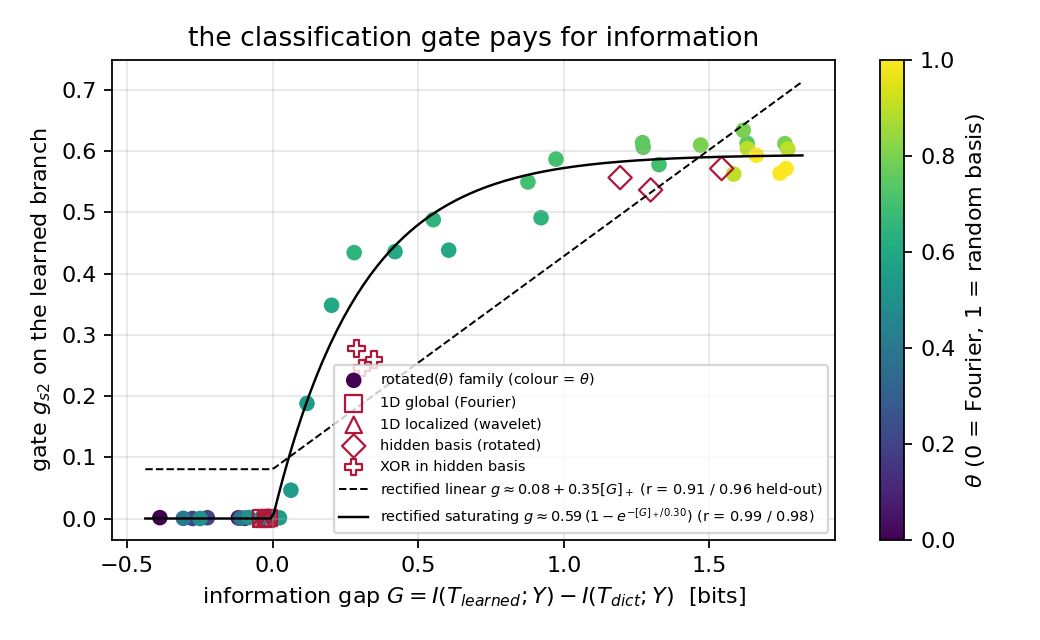
\includegraphics[width=0.78\linewidth]{gap_law.png}
\caption{The classification gate against the information gap. Filled circles: the rotated family, coloured by $\theta$; open markers: the four tasks of \cite{flob}, not used in the fit. Solid: Equation~\eqref{eq:gaplaw}; dashed: the rectified line.}
\label{fig:gaplaw}
\end{figure}

\section{Compressing toward the signal is not compressing toward the label}\label{sec:rr}
A codec keeps the coefficients with the most energy; a classifier needs the coefficients with the most class information. With the same pooled dictionary and the same head, selecting $K=16$ coefficients by energy against by class F-score gives Table~\ref{tab:rr} (three seeds). On the global (Fourier) task the two selections agree, because the discriminative tones are also the energetic ones. On the localized task energy selection keeps the carrier's spectral lines and discards the wavelet coefficients that encode \emph{position}, which is the class: accuracy drops from \rrLocTask{} to \rrLocEnergy{}. On the hidden-basis task both selections fail, because no dictionary coefficient carries the classes — which is exactly where Section~\ref{sec:gaplaw} showed the gate opening. Rate–distortion and rate–relevance \cite{tishby} are different objectives, and the gate measures the second, not the first.

\begin{table}[t]
\centering\small
\begin{tabular}{@{}lcc@{}}
\toprule
task & $K=16$ by energy & $K=16$ by class F-score \\
\midrule
1-D global (Fourier) & \rrGlobEnergy & \rrGlobTask \\
1-D localized (wavelet) & \rrLocEnergy & \rrLocTask \\
hidden basis (rotated) & \rrHidEnergy & \rrHidTask \\
\bottomrule
\end{tabular}
\caption{Test accuracy, mean over three seeds, same dictionary and head. What you keep decides.}
\label{tab:rr}
\end{table}

\section{The classification basis cannot be read back}\label{sec:symbolic}
If a learned unitary is worth something, one would like to \emph{name} it. We tried the simplest reading: after fixing the gauge (rows sorted by dominant frequency, row phases fixed), fit the closed form $U_{jk} = e^{-i a jk}/\sqrt N$ and report the normalized inner product with the best $a$. The untrained DFT scores \symDftFit{} at $a = \symDftA\cdot 2\pi/N$ — the reading works. A unitary trained with a compression prior plus cross-entropy scores \symSparseFit{}; one trained by cross-entropy alone from a random start scores \symCeFit{}, with \symCePure{} of its rows still pure sinusoids (Figure~\ref{fig:symbolic}). The task-trained basis is not a deformed Fourier transform that a formula could name: it is whatever separated the labels, and many bases do. This is the last row of Table~\ref{tab:correspondence}, and the reason Part~II exists. The same operation — read the learned part — becomes well-posed when the learned part is constrained by an operator rather than by a label.

\begin{figure}[t]
\centering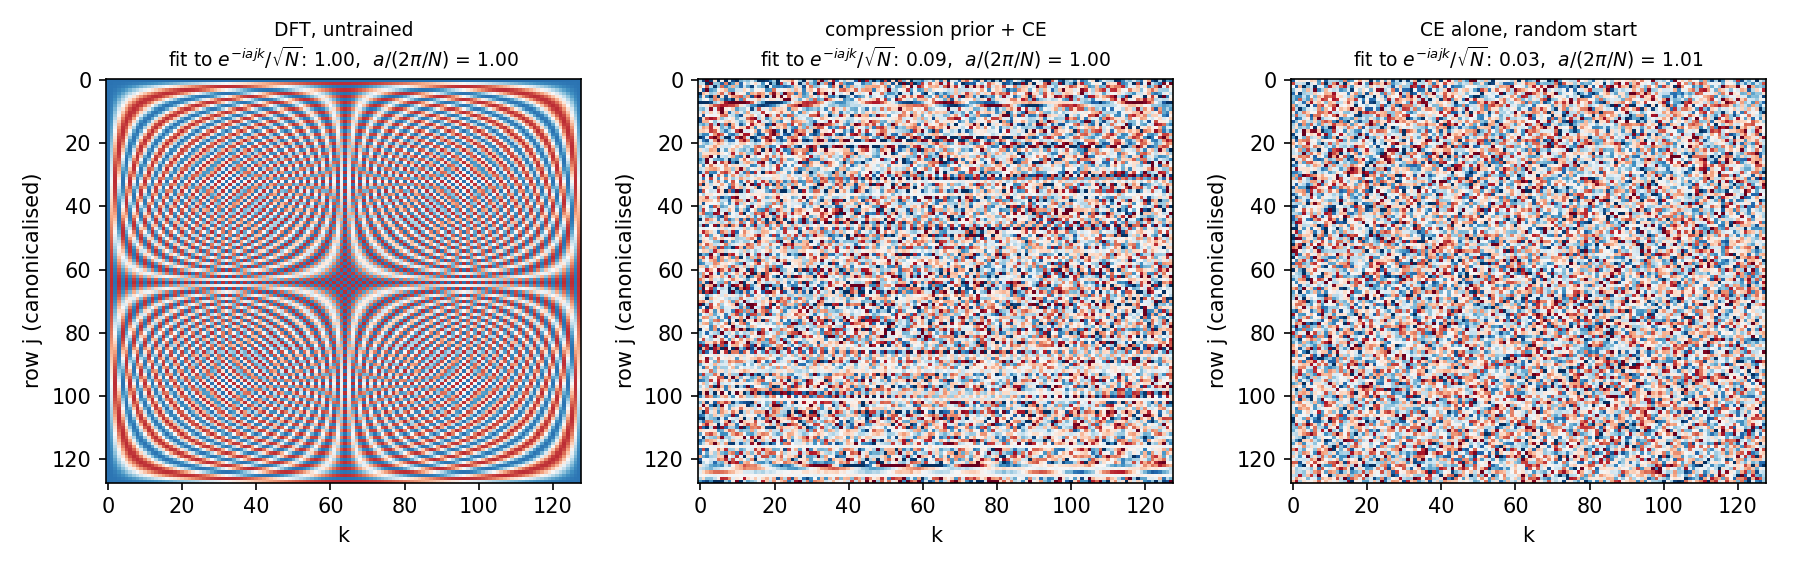
\includegraphics[width=\linewidth]{symbolic_U.png}
\caption{Real part of three unitaries after gauge canonicalisation, with the closed-form reading score. Left: the DFT reads exactly. Centre and right: task-trained bases do not.}
\label{fig:symbolic}
\end{figure}

%======================================================================
\part*{Part II — Physics: what the learned part says}
\section{Setup, and why each choice}\label{sec:setup}
\paragraph{Two families of operator.} We use two controlled one-dimensional families on a periodic grid of $N=64$ points on $[0,2\pi)$. The \emph{linear} family is diffusion with a spatially varying coefficient, $u_t = \partial_x(a(x)\,\partial_x u)$ with $a = 1 + \beta f(x)$, $f$ a fixed smooth normalized profile and $\beta$ the heterogeneity knob; $\beta=0$ is the constant-coefficient heat equation, whose eigenbasis is exactly Fourier. The \emph{nonlinear} family is viscous Burgers, $u_t = \nu u_{xx} - \varepsilon\,u u_x$ with $\nu = 0.05$ and $\varepsilon$ the nonlinearity knob; $\varepsilon = 0$ is the heat equation, $\varepsilon>0$ steepens fronts into shocks. Each family has a single knob that moves the physics away from the regime where a fixed spectral basis is exact, which is what a meter needs to be calibrated against.

\paragraph{Why divergence form and why $L = -G^{\mathsf T}\operatorname{diag}(a_f)G$.} Writing diffusion as $\partial_x(a\,\partial_x u)$ rather than $a\,u_{xx}$ keeps the operator self-adjoint, so it has a real spectrum and an orthonormal eigenbasis — the object the fixed and learned bases are compared against. The discretization mirrors that structure: $G$ is the periodic forward-difference matrix, $a_f$ is the coefficient on cell faces, and $L = -G^{\mathsf T}\operatorname{diag}(a_f)G$ is symmetric negative semi-definite by construction. It is also the discrete Sturm–Liouville operator, which is why the search family of Section~\ref{sec:discover} can be written in the same form.

\paragraph{Why a propagator.} A learned model predicts states, not operators, so the object to compare is the one-step map $u(t)\mapsto u(t+\Delta)$. For the linear family it is available in closed form, $P = \exp(L\Delta)$, and Equation~\eqref{eq:D} can be evaluated on it exactly. For the nonlinear family the propagator is the RK4 integration over $\Delta$, and the best linear approximation to it is what DMD fits.

\paragraph{Why RK4 with dealiasing and a long horizon.} Burgers is integrated with fourth-order Runge–Kutta at $\mathrm{d}t = 2\cdot10^{-3}$, spatial derivatives spectral, and the quadratic term dealiased by the $2/3$ rule so that the product $u u_x$ does not fold high wavenumbers back into the resolved band. Snapshots are taken every 85 steps ($\Delta = \wpDelta$): a horizon long enough for the nonlinearity to act on a single step, which is what makes the DMD residual a usable meter — with a short horizon every one-step map is nearly linear and the gate never has a reason to open (Section~\ref{sec:limits}). Initial conditions are smooth random superpositions of the first four harmonics at unit amplitude; \wpNtr{} training and \wpNte{} test trajectories of 32 snapshots per $\varepsilon$, plus \wpNte{} test trajectories at amplitude \wpAmpOod{} for the out-of-distribution test.

\section{A heterogeneity meter}\label{sec:hetero}
We sweep $\beta$ and evaluate Equation~\eqref{eq:D} for the fixed real Fourier basis and for the true eigenbasis $\Phi$ of $L$ — an oracle, removed in the next section. At $\beta=0$ Fourier diagonalizes $P$ exactly ($\Dm = 0.000$). As heterogeneity grows, $\Dm_{\mathrm{Fourier}}$ rises monotonically to \wpOneDmax{} at $\beta=4$, while $\Dm_\Phi$ stays at machine precision at every $\beta$; the alignment between $\Phi$ and Fourier — the mean energy of an eigenvector in its best single frequency — falls from $1.00$ to \wpOneAlignMin{} (Figure~\ref{fig:hetero}). The fixed basis is optimal exactly where the medium is homogeneous, and degrades in proportion to how far the physics has moved away from it. The failure of the fixed basis is the measurement.

\begin{figure}[t]
\centering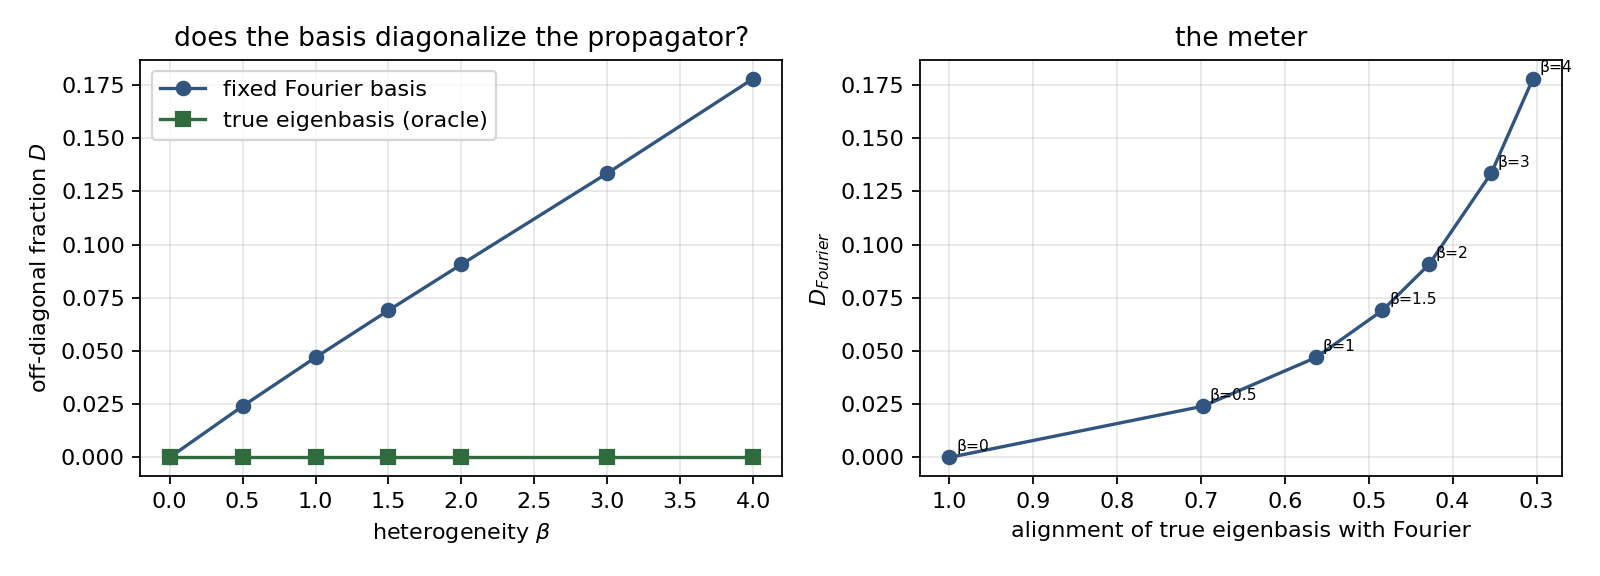
\includegraphics[width=\linewidth]{phys_wp1_meter.png}
\caption{Heterogeneity meter. Left: off-diagonal fraction of the propagator in the fixed Fourier basis (blue) and in the true eigenbasis (green) as the medium becomes heterogeneous. Right: the same Fourier curve as a meter, against the alignment between the true eigenbasis and Fourier.}
\label{fig:hetero}
\end{figure}

\section{Discovering the basis without an oracle}\label{sec:discover}
The oracle is the weak point of the previous section. Learning a free unitary is the classification failure mode of Section~\ref{sec:symbolic} — under-determined and drifting — so instead we search a \emph{structured} family: Sturm–Liouville operators $L(\theta) = -G^{\mathsf T}\operatorname{diag}(a_\theta)G$ with $a_\theta = 1 + $ a truncated Fourier series of $M$ harmonics ($2M$ parameters; $M=3$ or $5$). The objective is only Equation~\eqref{eq:D} on the true propagator: no labels, no trajectories, no oracle, started from Fourier ($\theta=0$), Powell's method with three restarts. The family is well motivated rather than arbitrary: the classical orthogonal bases (Fourier, Hermite, Legendre, Chebyshev) are eigenbases of Sturm–Liouville operators, so searching over them is searching over second-order differential operators. A degeneracy makes the operator, not the basis, the right thing to parametrize: at a fixed rank $K$ all polynomial families of degree $<K$ span the same subspace.

\paragraph{Result.} Off-diagonality falls from \wpOneDrange{} (Fourier) to \wpOneDiscD{} at every $\beta$, and the recovered coefficient matches the truth at correlation \wpOneCorr{} (Figure~\ref{fig:discover}). Eigenvectors are invariant under $a \to c\,a$, $c>0$, so $a$ is identifiable only up to a positive scale and recovery is scored after standardizing both profiles. The discovered basis is not merely a basis that works — it is the physics, readable as a coefficient field.

\paragraph{The meter detects its own mis-specification.} When the true $a(x)$ contains a harmonic outside the search family ($M=3$ while the truth has a fifth harmonic), recovery degrades: off-diagonality falls only \wpOneMisD{} and the recovered profile correlates \wpOneMisCorr{} with the truth. Widening the family to $M=5$ restores \wpOneDiscD{} and \wpOneCorr{}. The failure mode is mis-specification, not the method — and the objective value announces it by plateauing well above zero. This is the precise counterweight to Section~\ref{sec:depth}: structure is the lever, but wrong structure is worse than useless.

\begin{figure}[t]
\centering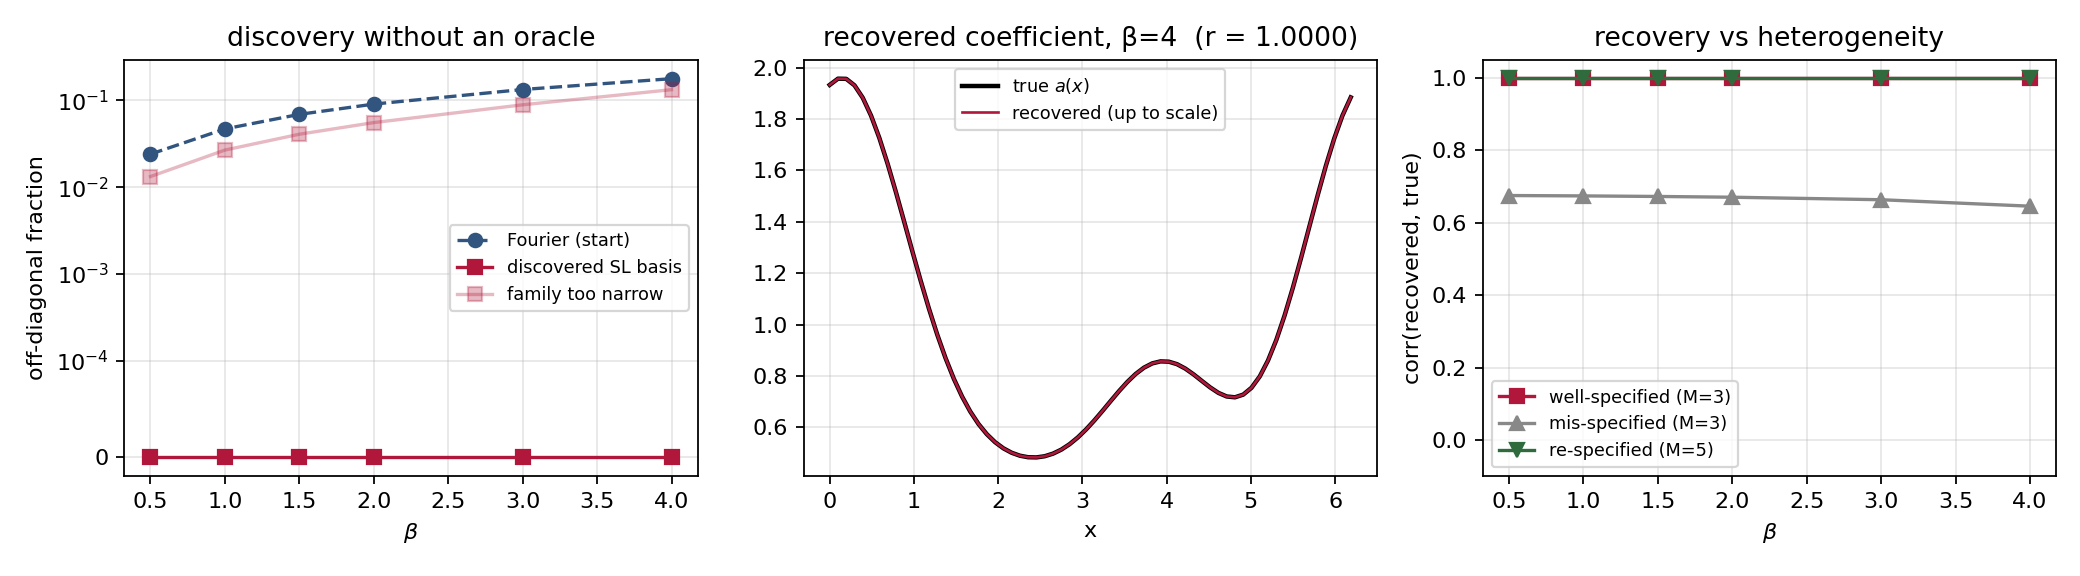
\includegraphics[width=\linewidth]{phys_wp1_discovery.png}
\caption{Discovering the basis. Left: the discovered Sturm–Liouville basis diagonalizes as well as the oracle, with no oracle; the pale curve is the same search with a family too narrow to contain the truth. Centre: the recovered coefficient over the true one. Right: recovery against heterogeneity for well-specified, mis-specified and re-specified families.}
\label{fig:discover}
\end{figure}

\section{A nonlinearity meter, and a gate that fires}\label{sec:nonlin}
We now move to Burgers and learn a one-step map over the horizon $\Delta$. The linear reference is the closed-form DMD propagator $A$ (Section~\ref{sec:meters}); its held-out residual is exactly what a Laplace-linear front-end cannot capture. On top we place the gated branch of Figure~\ref{fig:zoom-predictor}, $\hat u_1 = A u_0 + g\,\mathrm{NL}(u_0)$, with $A$ frozen and only the branch trained on the residual, $L_1$ weight $10^{-3}$ on $g$, weight decay $3\cdot10^{-5}$, 1500 full-batch epochs. The branch here is a black box (a two-layer perceptron); its gate is initialized open — starting it at zero makes $g\cdot\mathrm{NL}$ a dead saddle in which neither factor receives gradient.

Two things track $\varepsilon$ monotonically (Figure~\ref{fig:nonlin}). The DMD residual rises $0 \to \wpTwoResMax$: a clean nonlinearity meter. And the branch fires with a rectified, thresholded law — firing amplitude at or below \wpTwoFireShut{} up to $\varepsilon = \wpTwoEpsThresh$, where it also captures nothing out of sample, then \wpTwoFireFour{} at $\varepsilon = 0.4$, \wpTwoFireOne{} at $\varepsilon = 1$ and \wpTwoFireMax{} at $\varepsilon = 2$, rising roughly in proportion to the residual. That is the shape of Equation~\eqref{eq:gaplaw} without its saturation: shut until there is something to pay for, then proportional to it. When it fires it captures out of sample, removing \wpTwoCapRange{} of the DMD residual for $\varepsilon \ge 0.7$.

\begin{figure}[t]
\centering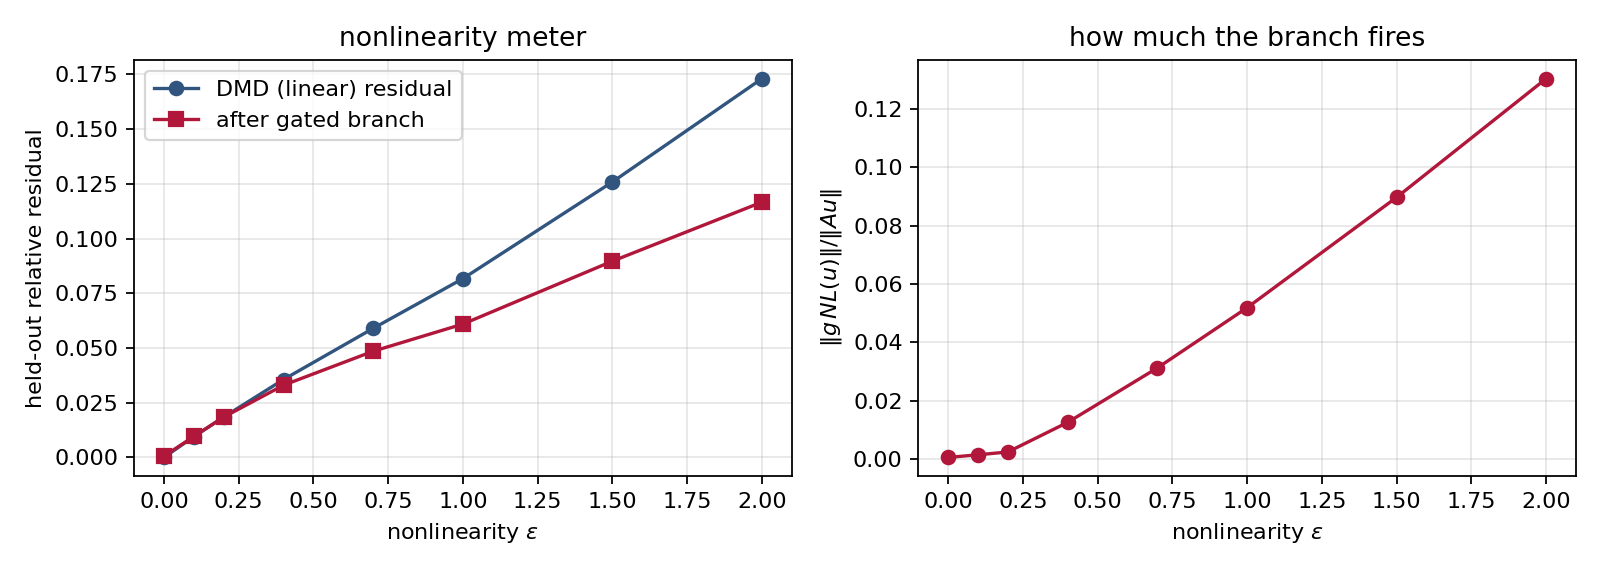
\includegraphics[width=\linewidth]{phys_wp2_meter.png}
\caption{Nonlinearity meter and gate. Left: DMD (linear) held-out residual against the nonlinearity knob, and the residual after the gated learned branch. Right: how much the branch fires — shut below threshold, then opening in proportion.}
\label{fig:nonlin}
\end{figure}

\section{Depth is not the lever; structure is}\label{sec:depth}
The black-box branch above leaves a good part of the DMD residual on the table. Since $u u_x$ is a low-order polynomial nonlinearity, the ceiling is one of generalization, not capacity. We therefore compare five branch designs on the identical frozen-DMD residual, same budget, scored by held-out capture (Table~\ref{tab:depth}, Figure~\ref{fig:depth}): a one-step perceptron; residual integrators of 4 and 8 stages, $v \leftarrow v + \tfrac1k f_i(v)$ with separate nets $f_i$, the neural-ODE-like way of adding depth; a structure-matched branch, a \emph{linear} map $W$ on the features $[u, u_x, u\,u_x]$; and a structured integrator, the same single $W$ applied in four sub-steps $v \leftarrow v + \tfrac14 W[v, v_x, v\,v_x]$ — structure plus depth, with no additional parameters.

\begin{table}[t]
\centering\small
\begin{tabular}{@{}lc@{}}
\toprule
nonlinear branch & mean held-out capture ($\varepsilon \ge 0.7$) \\
\midrule
one-step multi-layer perceptron (no depth) & \wpDepthMlp \\
residual integrator, 4 stages (neural-ODE-like) & \wpDepthResFour \\
residual integrator, 8 stages & \wpDepthResEight \\
structure-matched quadratic $[u, u_x, u\,u_x]$, one step & \wpDepthQuad \\
the same term, 4 sub-steps (structured integrator) & \wpDepthQuadInt \\
\bottomrule
\end{tabular}
\caption{Depth versus structure. Adding depth as a learned integrator helps; matching the form of the nonlinearity helps more, with a linear map and no hidden layer; sub-stepping that term closes the gap.}
\label{tab:depth}
\end{table}

\begin{figure}[t]
\centering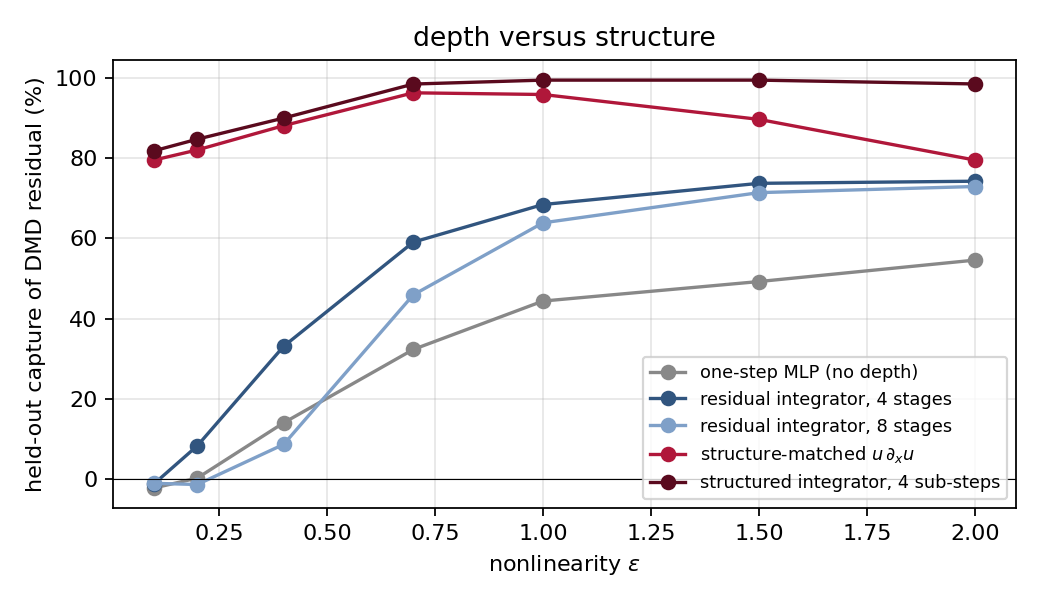
\includegraphics[width=0.7\linewidth]{depth_test.png}
\caption{Held-out capture of the DMD residual for five branch designs across the nonlinearity sweep.}
\label{fig:depth}
\end{figure}

Depth buys something — the 4-stage integrator improves on the perceptron, and 8 stages under-trains at the same budget — but the structure-matched branch, which has no hidden layer at all, captures more, and it does so already at $\varepsilon=0.1$ (\wpDepthQuadIntEpsOne{} for the structured integrator) where every black box is still shut (\wpDepthMlpEpsOne{}). The winning branch is not just better: it is the feature that sparse regression selects (next section). Capturing what a linear front-end misses and writing down the governing term are therefore the same operation, which is what makes the rest of Part~II possible. Whether that capture is worth anything beyond one step — and whether one explicit step of the right term is enough — is the question of Section~\ref{sec:extrap}.

\section{Reading the operator}\label{sec:sindy}
We estimate $u_t$ numerically (a forward difference of consecutive fine-step snapshots, not the analytic right-hand side), build a library of candidate terms $[u, u_x, u_{xx}, u_{xxx}, u^2, u u_x, u u_{xx}, (u_x)^2]$ with spectral derivatives, and run sequential thresholded least squares \cite{sindy,pdefind}, implemented directly.

The recovery is exact in the accessible regime (Figure~\ref{fig:sindy}): the diffusion coefficient is pinned at \wpSindyNuHat{} $= \nu$, the coefficient of $u u_x$ lies on the identity line $-\varepsilon$ (measured \wpSindyEpsList{} for $\varepsilon = 0.2, 0.4, 0.7, 1.0$), and every non-physical library term is driven to zero by the sparsity. Honest limit: for $\varepsilon \ge 1.5$ the nonlinear coefficient is under-estimated (\wpSindyEpsTwo{} against $-2.0$) and $\nu$ drifts to \wpSindyNuTwo. This is a resolution effect — strong shocks are under-resolved at $N=64$ and the numerical $u_t$ degrades where gradients steepen — not a failure of identification.

\begin{figure}[t]
\centering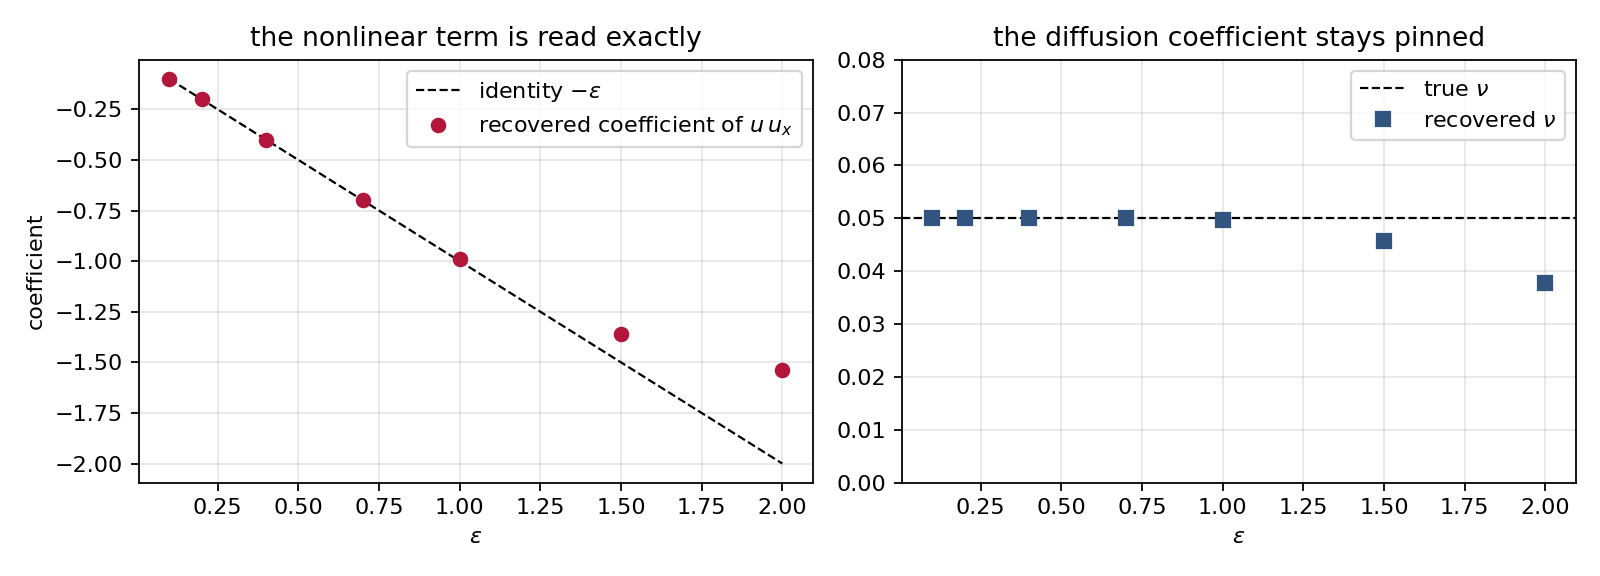
\includegraphics[width=\linewidth]{phys_wp3_sindy.png}
\caption{Reading the operator. Left: recovered coefficient of $u u_x$ against the ground truth $-\varepsilon$. Right: the linear (diffusion) coefficient stays pinned at $\nu$.}
\label{fig:sindy}
\end{figure}

\section{What the reading is worth: extrapolation}\label{sec:extrap}
Recovering an equation is only valuable if it buys something a black box cannot give. We test the sharpest version: one-step models sharing the same frozen DMD head, differing only in the nonlinear branch — (a) none, (b) the black-box perceptron, (c) the discovered $u u_x$ term in one explicit step, (d) the same term sub-stepped four times — all trained only on one-step pairs at $\varepsilon = 1.0$, then evaluated by a 30-step rollout (a horizon never seen) from in-distribution initial conditions, from initial conditions at \wpAmpOod$\times$ the training amplitude, and along an amplitude sweep with fresh initial conditions (Table~\ref{tab:extrap}, Figure~\ref{fig:extrap}).

\begin{table}[t]
\centering\small
\begin{tabular}{@{}lcc@{}}
\toprule
model & rollout error, in-distribution & rollout error, amplitude \wpAmpOod \\
\midrule
DMD linear only & \wpRollLinId & \wpRollLinOod \\
DMD + black-box branch & \wpRollMlpId & \wpRollMlpOod \\
DMD + discovered $u u_x$, one explicit step & \wpRollQuadId & \wpRollQuadOod \\
DMD + discovered $u u_x$, 4 sub-steps & \wpRollQuadIntId & \wpRollQuadIntOod \\
\bottomrule
\end{tabular}
\caption{Relative $L_2$ error at rollout step 30, seed 0, one-step training only. The structured integrator is \wpRollGainId$\times$ better than the linear model in horizon and \wpRollGainOod$\times$ at unseen amplitude; the black box is worse than the linear model on both.}
\label{tab:extrap}
\end{table}

\begin{figure}[t]
\centering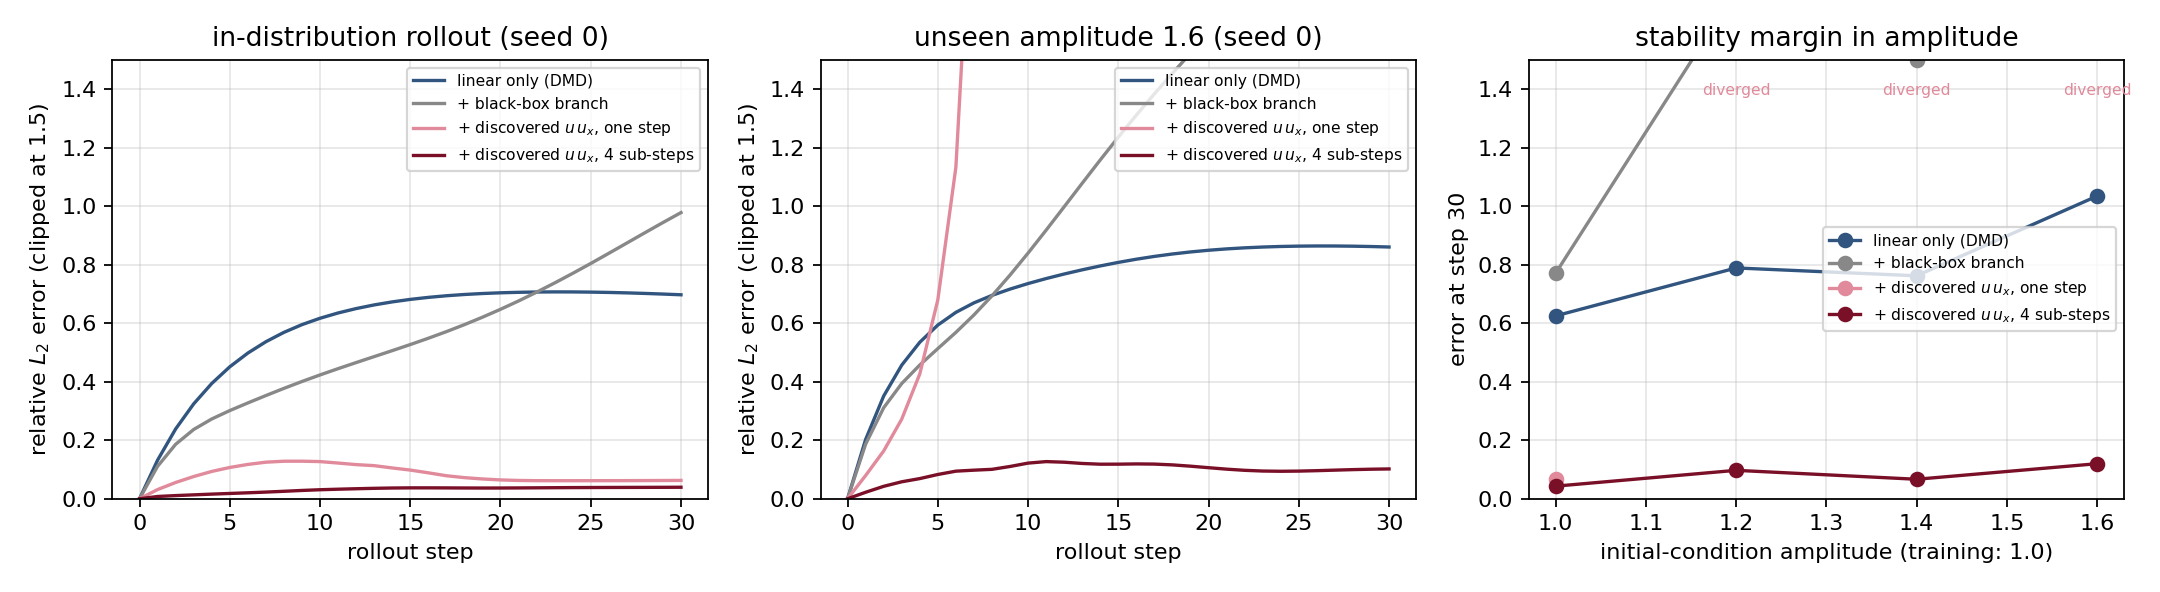
\includegraphics[width=\linewidth]{phys_wp4_rollout.png}
\caption{Extrapolation. Rollout error against step in distribution (left) and at amplitude \wpAmpOod{} (centre); error at step 30 against initial-condition amplitude, fresh initial conditions (right). Curves are clipped at 1.5; "diverged" marks errors that left the plot.}
\label{fig:extrap}
\end{figure}

Three things are visible. First, the black-box branch captured \wpTwoCapOne{} of the one-step residual at $\varepsilon=1$ and that capture does not compound: rolled out, it is \emph{worse} than the linear model it was meant to correct, in distribution and more so at larger amplitude, and it creates energy on \wpEnergyMlpIdMean{} of its in-distribution steps (\wpEnergyMlpOodMean{} out of distribution), which viscous Burgers never does. It learned a one-step correction on the training distribution, not an operator. Second, the discovered term applied in one explicit step extrapolates in horizon (error \wpRollQuadId{} at step 30) but has no stability margin in amplitude: at every amplitude above training it diverges (right panel). This is the behaviour of an explicit integrator pushed past its stability limit — the term is right, the step is too long for it — and it is a negative result we did not anticipate. Third, sub-stepping the same term restores the margin: the structured integrator stays at \wpRollQuadIntOod{} at \wpAmpOod$\times$ amplitude and below \wpAmpQuadIntMax{} across the sweep, while the linear model reaches \wpAmpLinMax{}, and it never creates energy. The structured term transfers because $u u_x$ is amplitude-covariant — under $u \to c u$ it scales as $c^2$ exactly as the physics does — so the physically correct term carries to a regime it never saw; but only a model that integrates that term, rather than applying it once, can use the covariance.

\section{Hardening: rollout training multiplies structure}\label{sec:harden}
Finally we ask whether training on rollouts rather than one-step pairs changes the picture. Rollout training is applied as fine-tuning on top of the converged one-step model, unrolling 5 steps with gradient clipping (300 epochs); three seeds, mean $\pm$ standard deviation, for the black box and for the structured integrator (Table~\ref{tab:harden}, Figure~\ref{fig:harden}). The one-step structured surrogate is included for completeness: rollout training improves it in distribution (\wpHardQuadStepOneId{} $\to$ \wpHardQuadStepRollId) and does not rescue it out of distribution, where it still diverges.

\paragraph{What the seeds vary.} The three seeds change the initialization of the nonlinear branch and the order of stochastic operations in training; they do \emph{not} resample the data. The training trajectories, the test initial conditions and the out-of-distribution initial conditions are fixed across seeds. The error bars therefore measure training variance, not data variance — the honest reading is "how reproducible is this model on this data", and the limitation is stated in Section~\ref{sec:limits}.

\begin{table}[t]
\centering\small
\begin{tabular}{@{}lcc@{}}
\toprule
model & in-distribution & unseen amplitude \\
\midrule
black-box branch, one-step trained & \wpHardMlpOneId & \wpHardMlpOneOod \\
black-box branch, + rollout training & \wpHardMlpRollId & \wpHardMlpRollOod \\
structured integrator, one-step trained & \wpHardQuadOneId & \wpHardQuadOneOod \\
structured integrator, + rollout training & \wpHardQuadRollId & \wpHardQuadRollOod \\
\bottomrule
\end{tabular}
\caption{Rollout error at step 30, three seeds (network initialization only). Rollout training improves the structured integrator \wpHardGain$\times$ in distribution and \wpHardGainOod$\times$ out of distribution, and the black box \wpHardMlpGain$\times$ and \wpHardMlpGainOod$\times$ — which leaves it worse than the linear model at unseen amplitude.}
\label{tab:harden}
\end{table}

\begin{figure}[t]
\centering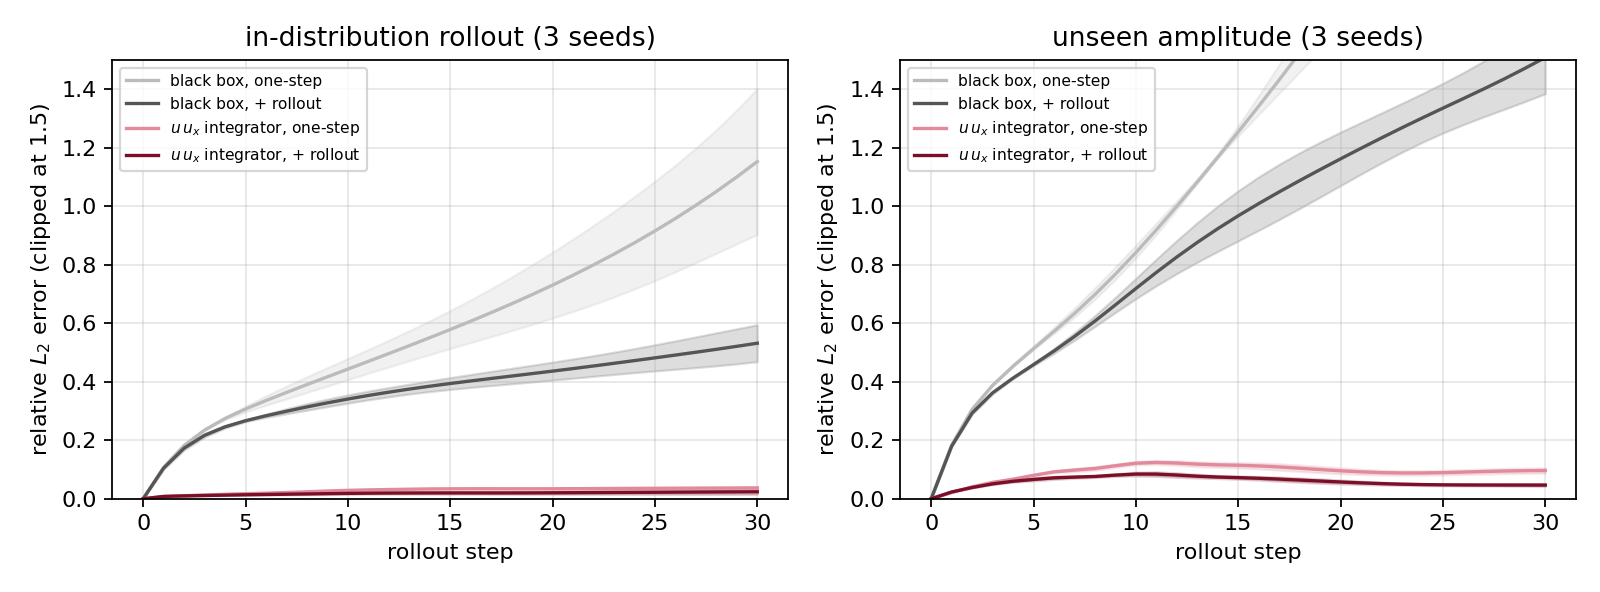
\includegraphics[width=\linewidth]{phys_wp4b_hardening.png}
\caption{Hardening, three seeds (shaded: $\pm 1$ s.d.; curves clipped at 1.5). Rollout training helps both models; only the one with the right structure ends up usable.}
\label{fig:harden}
\end{figure}

Rollout training is not a substitute for structure; it is a multiplier on it. It improves both models by a similar factor, and a similar factor applied to \wpHardMlpOneOod{} and to \wpHardQuadOneOod{} leaves one model unusable and the other at \wpHardQuadRollOod. The physical check — the fraction of rollout steps on which the predicted energy grows, which for viscous Burgers must be zero — discriminates here: the structured integrator never creates energy (\wpEnergyQuadIntId{} of steps in and out of distribution, before and after rollout training), the linear model never does either (\wpEnergyLinId), the black box does on \wpEnergyMlpIdMean{} of its in-distribution steps after one-step training and still on \wpEnergyMlpRollOod{} of its out-of-distribution steps after rollout training, and the one-step structured surrogate does on \wpEnergyQuadStepOod{} of its out-of-distribution steps as it diverges. We report it as a check, not as a metric optimized for: nothing in training penalized energy growth.

%======================================================================
\section{Related work}\label{sec:related}
Learning solution operators for PDEs is an active field; Fourier neural operators \cite{fno} are, in the language of this paper, the fixed-spectral branch promoted to an operator. Koopman theory and DMD \cite{mezic,schmid} are the learned-linear branch, and the reduced-order-modelling literature has long used them for prediction; Prony's method \cite{prony} is their ancestor for sums of exponentials. Sparse identification of nonlinear dynamics \cite{sindy} and PDE-FIND \cite{pdefind} provide the reading step of Section~\ref{sec:sindy}; we use them unmodified. Recovering a coefficient field from spectral data is the classical inverse-conductivity problem \cite{calderon}, a mature area; Section~\ref{sec:discover} is a small, well-specified parametric instance of it and claims no advance there. On the classification side, the information bottleneck \cite{tishby} is the formal statement that compressing toward a label and toward a signal are different objectives; Section~\ref{sec:gaplaw} measures a gate against that gap rather than proposing a new bound. It has been proved that invariant networks recover the Fourier transform of the underlying group and that the group is readable from the weights \cite{harmonics}; that result is stronger than anything we show about why classical bases appear, and we position our contribution as complementary and empirical. What we believe is not covered by the above is the packaging: a small set of calibrated meters with a shared shape — fixed structure plus measured failure — read through the \emph{same} gate in two objectives, together with the controls that keep them honest.

\section{Limitations and negative results}\label{sec:limits}
We state these explicitly, in the order they cost us time.

\paragraph{Two settings are two.} The gate law has the same functional form in classification and in physics. That is a coincidence of shape observed in two constructed families, not a universal law; we have not derived it, and $n=2$ does not license the word "universal". What we claim is narrower: in both settings the $L_1$-gated branch behaves as a rectified meter of what the branch adds, and that reading survived the controls below.

\paragraph{An artefact we had to remove.} The heterogeneity meter was first built from a prediction error with Fourier-smooth initial conditions. It produced a negative gap — Fourier apparently better than the eigenbasis — because those initial conditions let Fourier compress the data irrespective of the dynamics, and a full linear head made the basis irrelevant. Moving to the operator-level metric of Equation~\eqref{eq:D} removed the confound.

\paragraph{An unfair comparison we had to fix.} The first gated experiment trained a coupled network by stochastic gradient descent against a closed-form least-squares DMD and unsurprisingly lost, with a gate that did not behave as a meter. Freezing the DMD operator and training only the gated branch on its residual is what turned the gate into an instrument. A related recipe detail: a gate initialized at zero never opens, because $g\cdot\mathrm{NL}$ is then a saddle in which neither factor receives gradient; the gate must start open and be pushed shut by the penalty.

\paragraph{A horizon that hid the nonlinearity.} With a short snapshot interval every one-step map is nearly linear, the DMD residual is tiny and the $L_1$ penalty crushes the gate. The horizon must be long enough for the nonlinearity to act within one step.

\paragraph{A training recipe that diverges.} Rollout training from a cold network diverges (in an earlier run we observed exactly $1.000$ relative error, i.e. a collapsed prediction). It must be applied as fine-tuning on a converged one-step model, with gradient clipping.

\paragraph{The right term in one step is not enough.} We expected the one-step structured surrogate to extrapolate in amplitude because its term is amplitude-covariant. It does not: it diverges at every amplitude above training, like an explicit integrator past its stability limit. Sub-stepping the same term fixes it with no new parameters, but this was found, not designed, and the stability margin of the structured integrator has been mapped only up to \wpAmpOod$\times$ the training amplitude.

\paragraph{Seeds and data.} Out-of-distribution rollout numbers vary across seeds for the black box; single-seed out-of-distribution claims should not be trusted, which is why Section~\ref{sec:harden} reports error bars and Section~\ref{sec:extrap} should be read through them. The seeds vary the network, not the data; a data-resampled study would be the next step.

\paragraph{The information estimate is a bound.} $I(T;Y)$ is estimated by $H(Y)$ minus a held-out cross-entropy, a lower bound that depends on the head; we use the same small head for both branches so that the \emph{gap} is comparable, and we clip negative estimates to zero. A kNN or MINE estimator would be a useful cross-check.

\paragraph{Scope.} All physics experiments are one-dimensional, at $N=64$, with a single nonlinear term whose form we ourselves planted. Recovery correlations of $1.0000$ indicate a well-specified problem, not a difficult one: they validate the instrument, they do not demonstrate discovery on data whose answer is unknown. Strong shocks are under-resolved. The linear head is a fitted DMD operator, not the exact diffusion operator, which caps how far even the structured model transfers in amplitude. Structure preservation is verified a posteriori (energy monitoring) rather than imposed by construction; a symplectic or conservative parametrization is the natural next hardening step. The classification family is synthetic by design, so that the gap is controlled; the four benchmark tasks are the only uncontrolled points.

\section{Conclusion}
A gate that decides how much of a learned branch to use is worth exactly what the branch adds, and the two settings studied here agree on the shape of that price: nothing until there is something to pay for, then proportional. In classification the currency is information about the label, and the learned part cannot be read back because many bases pay the same. Inverting the objective to physical modelling makes the learned branch legible: the failure of a fixed spectral basis is a heterogeneity meter; the residual of a linear propagator is a nonlinearity meter; the branch that captures that residual best is not the deepest but the one with the right structure; that structure is the term sparse regression names; and putting the named term into the model — integrated, not applied once — is what buys extrapolation in horizon, in amplitude, and under rollout training, where structure is multiplied rather than replaced. The practical reading for a modeller is short: measure first whether your fixed front-end is failing and in which way, prefer a structured learned family over a free one, and treat the objective value itself as a mis-specification alarm.

\section{Reproducibility}\label{sec:repro}
NumPy/SciPy/PyTorch with fixed seeds, CPU only. Every experiment is a short deterministic script that regenerates the figures of the same name and writes its numbers to a JSON file in \texttt{results/}; every number in this paper is read from those files by \texttt{tools/make\_numbers.py}, which writes the macros used in the text, so a re-run that changes a number changes the paper. The classification scripts import the unmodified S1/S2/S3 code of \cite{flob}, vendored under \texttt{classification/flob\_lib/}. Trajectory generation for the Burgers sweep is cached in \texttt{results/cache/} and recomputed deterministically when absent.

\begin{table}[h]
\centering\small
\begin{tabularx}{\linewidth}{@{}l X@{}}
\toprule
section & script(s) \\
\midrule
\ref{sec:meters} DMD as Laplace & \texttt{physics/dmd\_laplace\_check.py} \\
\ref{sec:gaplaw} gate law in bits & \texttt{classification/gap\_law.py} \\
\ref{sec:rr} rate–relevance & \texttt{classification/rate\_relevance.py} \\
\ref{sec:symbolic} reading the basis & \texttt{classification/symbolic\_U.py} \\
\ref{sec:hetero}, \ref{sec:discover} heterogeneity, discovery & \texttt{physics/phys\_wp1.py} \\
\ref{sec:nonlin} nonlinearity meter & \texttt{physics/phys\_wp2.py} \\
\ref{sec:depth} depth versus structure & \texttt{physics/depth\_test.py} \\
\ref{sec:sindy} reading the operator & \texttt{physics/phys\_wp3\_sindy.py} \\
\ref{sec:extrap}, \ref{sec:harden} extrapolation, hardening & \texttt{physics/phys\_wp4\_rollout.py} \\
\bottomrule
\end{tabularx}
\caption{Section-to-script map. Shared numerics: \texttt{physics/common.py}, \texttt{physics/data.py}, \texttt{physics/models.py}.}
\end{table}

\begin{thebibliography}{99}\small
\bibitem{fno} Li, Z., Kovachki, N., Azizzadenesheli, K., et al.: Fourier Neural Operator for Parametric Partial Differential Equations. ICLR, 2021.
\bibitem{mezic} Mezić, I.: Spectral Properties of Dynamical Systems, Model Reduction and Decompositions. Nonlinear Dynamics 41, 2005.
\bibitem{schmid} Schmid, P.J.: Dynamic Mode Decomposition of Numerical and Experimental Data. Journal of Fluid Mechanics 656, 2010.
\bibitem{prony} de Prony, G.: Essai expérimental et analytique. Journal de l'École Polytechnique 1(22), 1795.
\bibitem{sindy} Brunton, S.L., Proctor, J.L., Kutz, J.N.: Discovering Governing Equations from Data by Sparse Identification of Nonlinear Dynamical Systems. PNAS 113(15), 2016.
\bibitem{pdefind} Rudy, S.H., Brunton, S.L., Proctor, J.L., Kutz, J.N.: Data-Driven Discovery of Partial Differential Equations. Science Advances 3(4), 2017.
\bibitem{calderon} Uhlmann, G.: Electrical Impedance Tomography and Calderón's Problem. Inverse Problems 25(12), 2009.
\bibitem{harmonics} Marchetti, G.L., Hillar, C., Kragic, D., Sanborn, S.: Harmonics of Learning: Universal Fourier Features Emerge in Invariant Networks. Proceedings of Machine Learning Research 247, 2024.
\bibitem{tishby} Tishby, N., Pereira, F.C., Bialek, W.: The Information Bottleneck Method. Allerton Conference, 1999.
\bibitem{flob} del Río Romero, J.C.: Fixed, Learned, or Both? A Machine-Learning Study of Self-Calibrating Gated Couplings of Transform Dictionaries and Learned Unitary Bases for Compact Signal Classification. Technical report (GitHub/Zenodo), 2026.
\end{thebibliography}
\end{document}
